\vspace{-6pt}
\section{Experiments}\label{sect:experiments}
\vspace{-4pt}

In this section, we evaluate the performance of DeDLOC in realistic collaborative training conditions. Our primary focus is on training models that are useful for a wide range of downstream tasks and thus would attract a large number of collaborators. One area that fits this description is self-supervised learning, i.e., learning reusable feature representations on large unlabeled datasets. First, we conduct controlled experiments on two popular self-supervised learning tasks in Sections~\ref{sect:exp_swav} and~\ref{sect:exp_albert}. Then, we set up a real-world collaborative training run with volunteers and report our findings in Section~\ref{sect:exp_bengali}.

\subsection{Self-supervised learning of visual representations}\label{sect:exp_swav}

Our first set of experiments uses SwAV~\cite{swav} --- a self-supervised learning technique that learns image representations by contrasting cluster assignments. Similarly to the original paper, we train the ResNet\nobreakdash-50~\cite{resnet} model on the ImageNet dataset~\cite{imagenet_cvpr09} without labels. Our experiments follow the recommended training configuration~\cite{swav,vissl}: 2+6 random crops, early prototype freezing and a queue with 3,840 samples for each worker, LARS~\cite{lars} optimizer, and 32,768 samples per batch across all workers. In this and further experiments, we use Hivemind~\cite{hivemind} to implement the infrastructure for decentralized averaging. We train with three hardware setups: \textsc{server}, \textsc{workstation} and \textsc{hybrid}. The \textsc{server} setup contains 8 workers, each with a single V100 GPU and 1 Gb/s symmetric bandwidth. In turn, the \textsc{workstation} setup consists of 16 nodes with 1080 Ti and 200 Mb/s bandwidth per worker. Finally, the \textsc{hybrid} setup combines both previous configurations for a total of 24 nodes. Unlike servers, workstation GPUs train in full precision because they do not support accelerated float16 computations~\cite{mixed_precision}.

We report learning curves for each hardware configuration in Figure~\ref{fig:swav_perf}. As expected, the \textsc{hybrid} setup converges the fastest, beating \textsc{server} and \textsc{workstation} setups by 40\% and 52\% accordingly. When used in a supervised setting (Section 4.1 from the original paper), the model learned in this setup achieves a comparable accuracy of 72.2\%.  Another important observation is that the workstation-only experiment achieves reasonable training throughput despite using dated hardware. To provide more insight into the performance of DeDLOC, we also measure the time it takes to run averaging in different configurations. We report the mean over 100 averaging rounds; the standard deviation was below 1\% in all setups. As demonstrated in Table~\ref{tab:averaging_perf}, adaptive averaging does not affect the performance for homogeneous setups while running $1.9$ times faster on the hybrid infrastructure.

\vspace{4pt}
\begin{minipage}[b][][b]{0.5\textwidth}
\centering
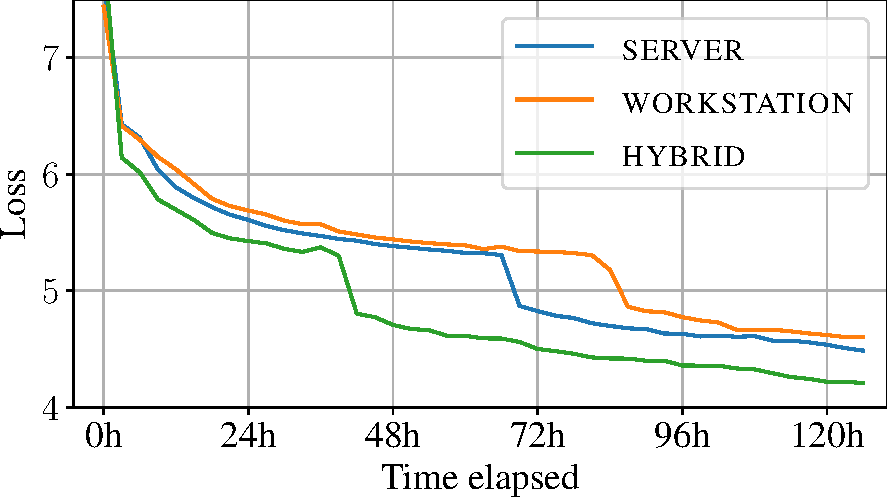
\includegraphics[height=100px]{resources/swav.pdf}
\captionof{figure}{SwAV pretraining performance.}
\label{fig:swav_perf}
\end{minipage}
\begin{minipage}[b][][b]{0.49\textwidth}
\centering
\renewcommand{\arraystretch}{1.2}
\begin{tabular}{lccc}
\toprule
\multicolumn{1}{c}{\multirow{2}{*}{Setup}} & \multicolumn{3}{c}{Algorithm} \\
 & AR & PS & Ours             \\ 
\midrule
A: 8x1Gb/s & \textbf{1.19} & 4.73 & 1.20 \\
B: 16x0.2Gb/s & \textbf{5.3} & 39.6 & \textbf{5.3} \\
C: A + B& 5.69 & 14.1 & \textbf{2.96} \\
D: B + 1x2.5Gb/s & 5.3 & 3.22 & \textbf{3.18} \\
\bottomrule
\end{tabular}
\vspace{8pt}
\captionof{table}{ResNet-50 averaging performance.}
\label{tab:averaging_perf}
\end{minipage}
\vspace{-4pt}

\subsection{Self-supervised pretraining for language understanding}
\label{sect:exp_albert}

Next, we investigate how collaborative training performs for more complex models. In this experiment, we pretrain the ALBERT-large~\cite{albert} masked language model on the WikiText-103 dataset~\cite{wikitext103}. We chose this setup for two reasons: first, ALBERT is very sensitive to the choice of hyperparameters, and specifically batch size, even more than regular Transformers~\cite{trainingtips}. This makes it easier to verify that DeDLOC can reproduce the training conditions of regular data-parallel training. Second, because of weight sharing, training ALBERT is relatively more compute- and less communication-intensive than regular BERT~\cite{bert}, which makes it possible to train with lower bandwidth.
\nocite{paszke2019pytorch}

As before, we follow the exact training configuration from the original paper, but use GPUs instead of TPUs. We use the implementation of ALBERT from the \texttt{transformers} library~\cite{wolf-etal-2020-transformers}. We run all experiments on cloud instances with Tesla T4 GPUs and report the training loss as a function of time, similarly to~\cite{lin2020multinode,switch}. In order to evaluate how DeDLOC performs with different network speeds, we consider the following setups on the same platform with controlled conditions:
\begin{itemize}[leftmargin=*]
   \item \textbf{High-bandwidth:} 16 workers, each with Tesla T4 and 25 Gb/s symmetric bandwidth;
    \item \textbf{Heterogeneous:} same, but with 4x 200 Mb/s, 8x 100 Mb/s and 4x 50 Mb/s bandwidths;
    \item \textbf{Heterogeneous + load balancing:} like Heterogeneous, but with adaptive averaging (Section~\ref{sect:method_algorithm});
    \item \textbf{Auxiliary peers:} the previous setup with 4 additional CPU-only peers at 1 Gb/s bandwidth.
    \item \textbf{Time-varying:} same as previous, but with 8 additional peers at 100 Mb/s. The extra peers are training part-time, jointly alternating between 8 hours of training and 8 hours of downtime.
\end{itemize}
\pagebreak[0]

\begin{minipage}[b][][b]{0.65\textwidth}
\centering
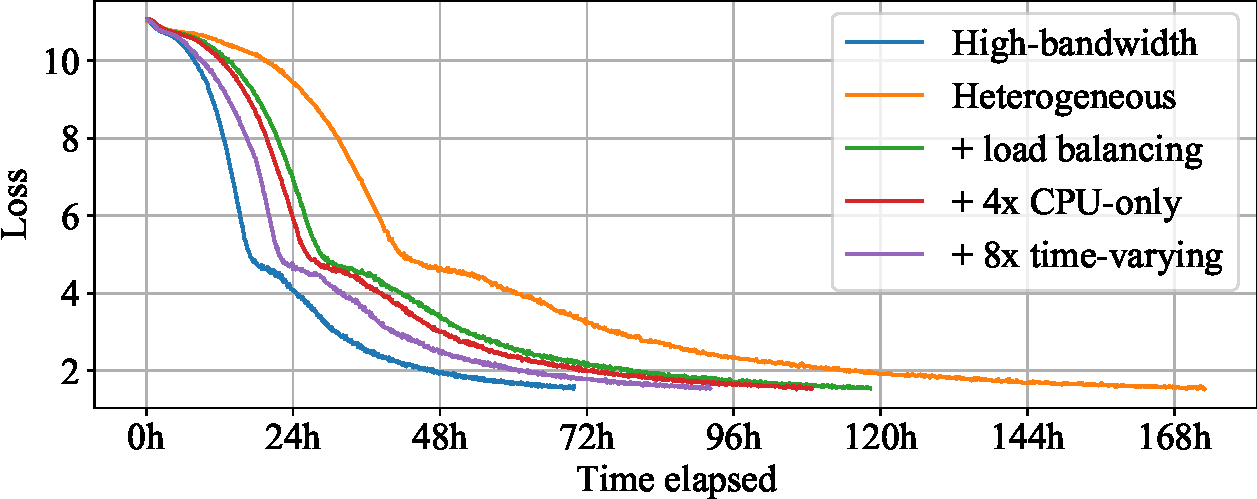
\includegraphics[width=\textwidth]{resources/convergence_albert.pdf}
\vspace{-14pt}
\captionof{figure}{ALBERT pretraining performance.}
\label{fig:albert_perf}
\end{minipage}
\begin{minipage}[b][][b]{0.32\textwidth}
\centering
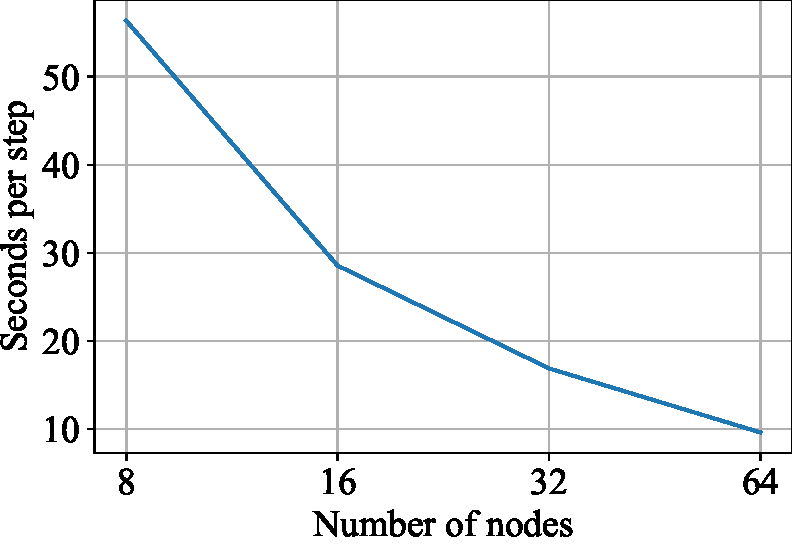
\includegraphics[width=\textwidth]{resources/albert_scalability.pdf}
\vspace{-14pt}
\captionof{figure}{Scalability measurements for ALBERT pretraining.}
\label{fig:albert_scalability}
\end{minipage}

As one can see in Figure~\ref{fig:albert_perf}, naïve training with low-bandwidth peers results in an~$\approx$ 2.5x slowdown compared to high-bandwidth ones. Enabling load balancing accelerates that setup by $\approx47\%$. This effect grows to over 60\% when adding 4 auxiliary peers. Finally, adding 8 part-time peers allows the collaboration to train at 74\% the speed of the high-bandwidth setup without sacrificing the training stability. This turns the latter setup into a viable alternative to traditional distributed training without the need for expensive infrastructure (see the cost analysis in Appendix~\ref{appendix:cost_analysis}). In addition, we demonstrate the high scalability of DeDLOC in Figure~\ref{fig:albert_scalability}, which was obtained by running the same experiment with a varying number of nodes and measuring the time between gradient descent steps. 

\vspace{-6pt}
\subsection{Real-world collaborative training}\label{sect:exp_bengali}
\vspace{-4pt}

For our final evaluation, we organized an actual collaborative training run with volunteer participants, who were asked to pretrain a Transformer masked language model for the Bengali language. This task was chosen deliberately to show the benefits of collaborative training: Bengali has over 230M native speakers who can benefit from recent advances in NLP, but there are few pretrained models available for this language.
We recruited 30 Bengali-speaking volunteers and 10 outside collaborators. All participants received instructions for contributing with free cloud platforms and access to the code for training on local computers. To avoid bias, we did not encourage any specific form of participation: volunteers were free to choose what hardware they contributed and for how long.

Specifically, we trained the ALBERT-large model on Wikipedia and the Bengali part of the OSCAR~\cite{Oscar} multilingual corpus. The model was named sahajBERT after conducting a poll among the participants. We adapted our preprocessing by following the best practices for the Bengali language described in Appendix~\ref{appendix:bn_albert_tokenizer}. To stream from a mix of Wikipedia and OSCAR, the training process iteratively sampled examples from one or the other dataset, as described in Section~\ref{sect:method_system_design}. We accounted for uneven size and quality of data by oversampling Wikipedia by a factor of 2, which resulted in mixing probabilities of 0.23 for Wikipedia and 0.77 for OSCAR. Other hyperparameters were set to the same values as in Section~\ref{sect:exp_albert}. Also, in Appendix~\ref{appendix:xl} we report the results of sahajBERT-XL --- a four times larger model with a specialized architecture that used both GPU and TPU resources.

\begin{figure}[b]
\vspace{-14pt}
% \captionsetup[subfigure]{belowskip=-1pt}
\noindent
\centering
\begin{subfigure}[t]{0.37\textwidth}
\centering
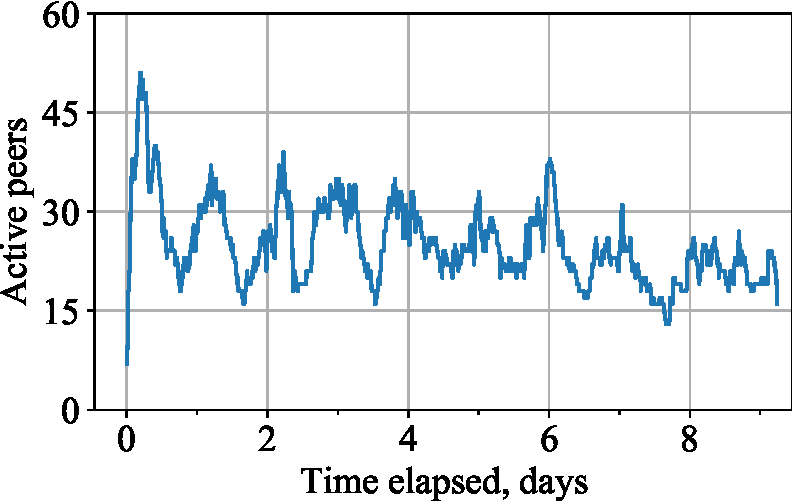
\includegraphics[width=\textwidth]{resources/peer_activity.pdf}
\caption{Collaboration activity.}
\label{fig:activity}
\end{subfigure}
\begin{subfigure}[t]{0.3\textwidth}
\centering
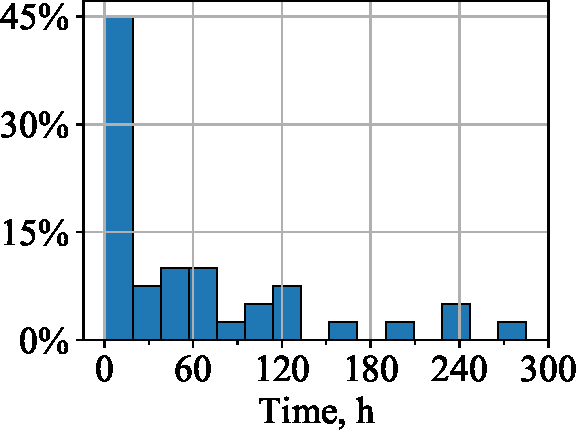
\includegraphics[width=\textwidth]{resources/contrib_hist.pdf}
\caption{Participation time histogram.}
\label{fig:contrib}
\end{subfigure}
\begin{subfigure}[t]{0.3\textwidth}
\centering
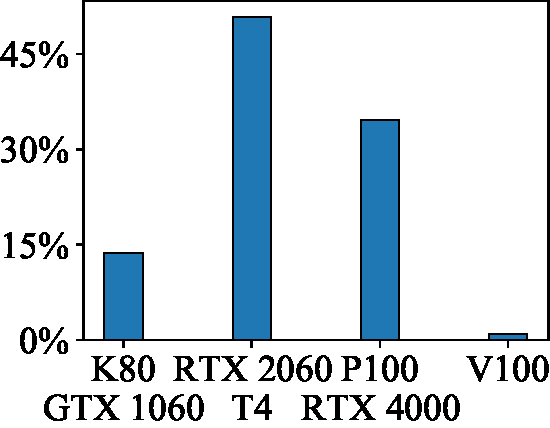
\includegraphics[width=\textwidth]{resources/gpu_hist.pdf}
\caption{Summary of volunteer hardware with example GPUs.}
\label{fig:device}
\end{subfigure}
\vspace{-4pt}
\caption{Collaborative experiment summary.}
\end{figure}


In total, the 40 volunteers contributed compute time from 91 unique devices, most of which were running episodically. Figure~\ref{fig:contrib} shows that although the median GPU time contributed by volunteers across all devices was $\approx$ 1.5 days, some participants ran the training script on several devices, attaining more than 200 hours over the duration of the experiment. With the exception of the start and the end of the collaborative run, the number of simultaneously active devices mostly varied between 15 and 35 depending on the local time. There was less activity in the last 3 days, likely because the volunteers could see that the model has converged on a public Weights \& Biases~\cite{wandb} dashboard.

As depicted in Figure~\ref{fig:device}, individual device performance varied significantly among the collaborators. Along with the resources provided by participants, we also used 16 preemptible single-GPU cloud T4 instances for training.
We have estimated that the average volunteer device consumed 6.95 GB of network traffic per hour of training. While this bandwidth usage is by no means insignificant, it is comparable with cloud gaming~\cite{google_stadia} or high-quality video streaming~\cite{netflix}.

The model converged after 8 days of training, which is 1.8x as fast as regular distributed training with 8 V100 GPUs that we ran as a baseline; Figure~\ref{fig:collab_loss} displays the convergence plots for both setups. At the same time, the stepwise learning curves of the two runs were virtually identical (see Appendix~\ref{appendix:stepwise_learning_curves}), which supports our hypothesis that training with DeDLOC is equivalent to a regular large-batch SGD.
 
\vspace{2pt}
\begin{minipage}[b]{0.49\textwidth}
\centering
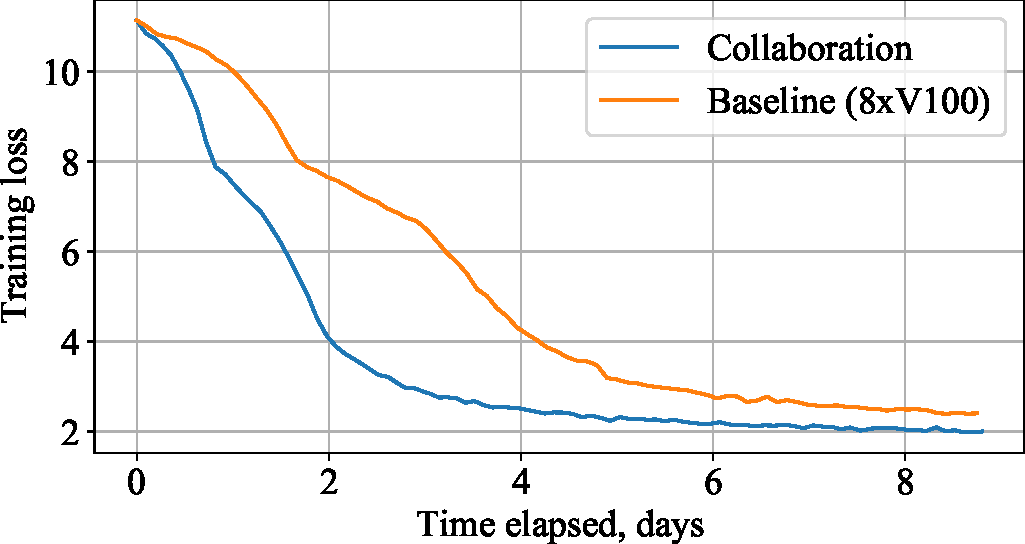
\includegraphics[width=0.95\linewidth]{resources/loss_collab_bengali.pdf}
\vspace{-4pt}
\captionof{figure}{Training progress of sahajBERT.}
\label{fig:collab_loss}
\end{minipage}
\begin{minipage}[b]{0.5\textwidth}
\setlength{\tabcolsep}{2pt}
\renewcommand{\arraystretch}{1.2}
\begin{tabular}{lcc}
\toprule
Model  & Wikiann F1 &NCC Accuracy \\
\midrule
bnRoBERTa           & 82.32 $\pm$ 0.67 &  80.94 $\pm$ 0.45 \\
IndicBERT           & 92.52 $\pm$ 0.45 &  74.46 $\pm$ 1.91 \\
XLM-R               & 96.48 $\pm$ 0.22 &  90.05 $\pm$ 0.38 \\
\midrule
sahajBERT           & 95.45 $\pm$ 0.53 &  91.97 $\pm$ 0.47 \\
sahajBERT-XL        & \bf 96.59 $\pm$ 0.26 & \bf 92.91 $\pm$ 0.43 \\
\bottomrule
\end{tabular}
\captionof{table}{Downstream evaluation results.}
\label{tab:downstream}
\end{minipage}

Finally, we compared the Bengali language representations of sahajBERT with those of other pretrained models on several downstream applications. The first model is XLM-R Large~\cite{xlmr} --- a cross-lingual Transformer-based masked language model that was pretrained on 100 languages and remains a strong baseline for multilingual representation learning. Similarly to sahajBERT, the second model, IndicBERT~\cite{kakwani-etal-2020-indicnlpsuite}, is also based on the ALBERT architecture; however, it was pretrained on 12 languages, including Bengali and Indian English. The third model, bnRoBERTa~\cite{jain2020indictransformers}, is a RoBERTa architecture trained on a monolingual Bengali corpus. We evaluate the model quality on two tasks: WikiANN~\cite{pan-etal-2017-cross} named entity recognition dataset and Soham News Category Classification benchmark from IndicGLUE~\cite{kakwani-etal-2020-indicnlpsuite}. For a detailed description of the setup, refer to Appendix~\ref{appendix:exp_bengali_evaluation}.

As shown in Table~\ref{tab:downstream}, sahajBERT performs comparably to three strong baselines despite being pretrained in a heterogeneous and highly unstable setting.
Notably, our collaboratively trained model outperforms two specialized monolingual baselines and demonstrates competitive results to XLM-R Large, even though the latter has significantly more parameters (560 million instead of 17 million) and was trained on five hundred high-performance data center GPUs instead of tens of low-cost or even free-tier accelerators.
This result confirms previous findings on the benefits of parameter sharing  that were made by authors of ALBERT. Also, it highlights one additional advantage of such architectures: specifically, one can train a high-quality representation model in a communication-constrained setting (for instance, over the Internet) without facing noticeable data transfer bottlenecks.